\section{Ejercicio 3}
\subsection{El Problema}
En este problema interesa construir una muralla para salvar lugares históricos.

Por un lado, nos brindan H puntos donde se encuentran estos lugares históricos que nos gustaría salvar. Por el otro, nos dicen la ubicación de E edificios tomados por enemigos que no queremos mantener dentro de la nueva muralla.

Nos piden un algoritmo polinomial (preferentemente \O{(H+E)^4}) que compute el polígono convexo que contenga a la mayor cantidad de edificios históricos, pero que no contenga ningún edificio tomado por enemigos. En particular interesa la cantidad máxima de edificios que se pueden salvar y no el polígono en sí.

Desde ahora llamaremos puntos \textit{buenos} a los lugares históricos a salvar y \textit{malos} a los que pertenecen a los edificios tomados por enemigos.

\subsection{Estrategia}
Para resolver este problema, planteamos el siguiente esquema:

Si supiéramos cuál es el punto que se encuentra más abajo a la izquierda del polígono solución, entonces podemos calcular la cápsula convexa pedida con este punto como referencia. Este punto será llamado \textit{\textbf{pivot}}.

Notemos que si el polígono solución tiene $k > 2$ vértices, puede ser dividido en $k - 2$ triángulos con vértices \textit{pivot}-$punto_i$-$punto_{i+1}$. Vamos a querer conocer cuantos puntos buenos y malos tiene cada uno de estos triángulos, para usar esta información más tarde.

Por ejemplo, dada la siguiente imagen, donde los puntos verdes son los buenos y el rojo el único malo.

\begin{figure}[H]\centering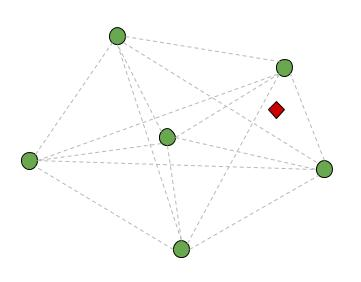
\includegraphics[scale=0.7]{Imagenes/ej3/Imagen_A.jpg}\caption{Posible input del problema}\end{figure}

Puede formarse un triángulo que contiene un punto bueno adentro. Y puede formarse uno que contiene un punto malo adentro.

\miniig{Imagenes/ej3/Imagen_B.jpg}{Posible triángulo a formar con puntos buenos dentro}{Imagenes/ej3/Imagen_C.jpg}{Posible triángulo a formar con puntos malos dentro}

Supongamos ahora que ya encontramos el punto \textit{pivot}, y que calculamos los triángulos y sus contenidos. Veamos ahora cómo construir el polígono buscado:

Si H = 0, no hay polígono que construir, si H = 1, ese punto será la cápsula máxima, si H = 2, entonces el segmento entre ellos será solución, pues no existen 3 puntos colineales.

Veamos el caso $H \geq 3$:

En primer medida vamos a ordenar los H puntos respecto al ángulo con el \textit{pivot}, en sentido anti-horario.

\begin{figure}[H]\centering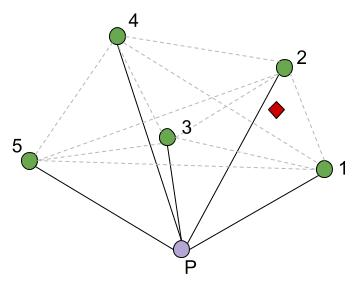
\includegraphics[scale=0.7]{Imagenes/ej3/Imagen_D.jpg}\caption{Puntos ordenados por ángulo respecto al pivot, en sentido anti-horario}\end{figure}

Además, como no existen 3 puntos colineales, cualquier segmento desde \textit{pivot} hacia los demás puntos son candidatos a solución.

La idea será la siguiente: para cada punto $X$ distinto al \textit{pivot}, armar todos los triángulos posibles con otros puntos buenos anteriores, que llamaremos $Y$. Los siguientes son los triángulos posibles desde el punto 4:

\begin{figure}[H]\centering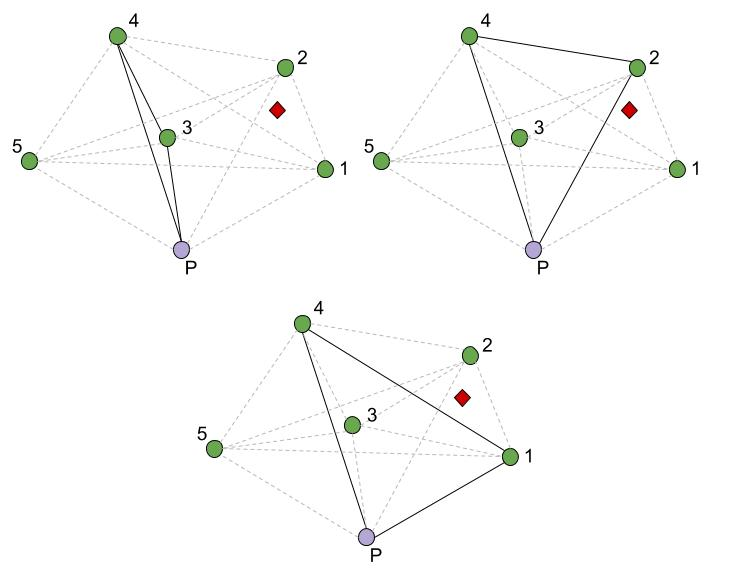
\includegraphics[scale=0.5]{Imagenes/ej3/Imagen_E.jpg}\caption{Triángulos posibles desde el punto 4}\end{figure}

Si uno de estos triángulos tiene dentro un punto malo, lo descartamos. Si no es así, calculamos recursivamente los posibles triángulos desde $Y$ que además sean convexos respecto al triángulo \textit{pivot}-$X$-$Y$ y no tengan dentro puntos malos. Si seguimos tomando a $X$ como 4 y tomamos a $Y$ como 3, estos serían los posibles sub triángulos.

\ig{Imagenes/ej3/Imagen_F.jpg}{Posibles sub triángulos con X = 4 e Y = 3}

Cabe aclarar que ninguno de estos triángulos forma una figura convexa con el triángulo P-4-3, por lo que no serán tenidos en cuenta para la solución final.

Ahora, en cada uno de estos pasos, podemos ir contando la cantidad de cantidad de puntos buenos que quedan dentro del polígono que estamos armando. De esta forma vamos a encontrar el mejor polígono posible para el \textit{pivot} elegido. Lo único que falta ahora es repetir el algoritmo eligiendo a un \textit{pivot} nuevo en cada iteración y devolver el máximo entre todas las iteraciones.

\subsection{Implementación}
En primera instancia precomputamos todas las triangulaciones posibles desde cada punto. Para cada uno de estos, guardamos además cuántos puntos buenos y cuántos malos tienen dentro cada uno. Por motivos de eficiencia, al tener que reordenar el arreglo de puntos buenos de acuerdo al \textit{pivot} en cada iteración, guardamos en este el índice por el cual indexar el precómputo de los triángulos.

La forma que decidimos implementar el algoritmo descrito previamente fue la siguiente: a partir de un punto cualquiera (distinto al \textit{pivot}), recorrer todos los que están entre este y el \textit{pivot}. Recordemos que estos ya se encuentran ordenados.

De esta manera llamaremos:
\begin{itemize}
  \item \textit{current} = cada uno de los puntos desde el tercero en adelante, siendo el primero el \textit{pivot}.

  \item \textit{prevLast} = cada uno de los puntos entre \textit{pivot} y current - 1.

  \item \textit{last} = cada uno de los puntos entre prevLast + 1 y current.
\end{itemize}

Si los tres puntos se encuentran en sentido anti-horario respeto a \textit{last}, entonces mantienen el atributo de convexidad buscado, por lo tanto, la configuración es un candidato válido.

Dadas estas definiciones, se derivan los triángulos con vértices \textit{pivot}-\textit{last}-\textit{current} (PLC) y \textit{pivot}-\textit{prevLast}-\textit{last} (PPL).

Si en PLC hay algún punto \textit{malo}, no nos sirve y lo descartamos. Si no contiene ningún punto \textit{malo}, entonces una posible solución será igual a la cantidad de puntos \textit{buenos} dentro de PLC + 1 (agregar \textit{current} al polígono) + la mejor solución hallada en PPL (este caso es recursivo). Nuestro caso base es siempre es 2, es decir el \textit{pivot} + cualquier otro punto.

Notamos también que tenemos subproblemas repetidos, que no queremos recalcular cada vez, con lo cual, podemos guardarlos en un \textbf{memo}. Las claves de este serán los puntos \textit{last} y \textit{current} e indicarán la máxima cantidad de puntos que se salvan usando el triángulo PLC para toda posible configuración.

Alcanza entonces con devolver el máximo de estos cálculos.

Finalmente, tenemos que eliminar el \textit{pivot} de los puntos buenos y repetir el proceso para contemplar todos los casos, pues partimos de la hipótesis de que el \textit{pivot} pertenece al polígono solución.

\subsubsection{Complejidad}
Como mencionamos previamente, lo primero que hacemos es calcular todos los triángulos que se forman con los puntos buenos. En total son \O{N^3} triangulos (elijo 1 vértice de los N, otro de los N-1 restantes y uno más de los N-2 finales).

Por cada triángulo, calculamos la cantidad de puntos buenos y malos dentro de él. Es decir que para cada triángulo ABC, por cada punto P creamos 4 segmentos AB, AC, BC, PK (\O{1}) y calculamos la cantidad de intersecciones entre ellos. Si la cantidad de intersecciones es par, entonces el punto está afuera, si no, está adentro. K es un punto que calculamos al principio que está fuera de todo posible triángulo \O{N}. La intersección de segmentos son simples cuentas, y por lo tanto \O{1}. En definitiva el costo de esta etapa es \O{N + N^3 * N} = \O{N^4}.

Una vez calculado esto, aplicamos el algoritmo descrito previamente. Tenemos \O{H} $\in$ \O{N} puntos \textit{buenos} sobre los que iterar. Por cada uno de estos, ordenamos los puntos (buscar el \textit{pivot} y ordenar según el ángulo, \O{N + N log(N)}), luego iterar los índices \textit{current} entre 2 y H (\O{N}), \textit{prevLast} entre 0 y current (\O{N}) y \textit{last} entre prevLast + 1 y current (\O{N}), esto es \O{N^3}.

Entonces por cada punto \textit{bueno}, tardamos \O{N log(N) + N^3}. Como tenemos \O{N} puntos buenos que iterar, la complejidad de esta parte es \O{N^4}.

Finalmente, el problema se resuelve en 2 etapas de costo \O{N^4 + N^4}, lo que se resume en \O{N^4} como se pedía.

\subsection{Puntaje}
El peso otorgado a este ejercicio es: 10
